%==============================================================
%  Warehouse That Reroutes Itself
%  Multi-Agent Robot Fleet Coordination Under Dynamic Disruptions
%  Foundations of AI -- Case Study -- Group 10
%
%  Compile:  pdflatex warehouse_reroutes_itself.tex   (run TWICE --
%            TikZ "remember picture" and the slide counter need it)
%==============================================================

\documentclass[aspectratio=169,10pt,xcolor=table]{beamer}

\usepackage[T1]{fontenc}
\usepackage{lmodern}
\usepackage{amsmath}
\usepackage{amssymb}
\usepackage{booktabs}
\usepackage{array}
\usepackage{ragged2e}
\usepackage{tikz}
\usetikzlibrary{arrows.meta,positioning,calc}

%--------------------------------------------------------------
%  COLOUR PALETTE -- Amrita maroon
%--------------------------------------------------------------
\definecolor{AmritaMaroon}{RGB}{122,16,38}
\definecolor{MaroonLight}{RGB}{166,25,46}
\definecolor{MaroonTint}{RGB}{247,238,240}
\definecolor{Charcoal}{RGB}{51,51,51}
\definecolor{SoftGray}{RGB}{238,238,238}
\definecolor{MidGray}{RGB}{120,120,120}

%--------------------------------------------------------------
%  THEME
%--------------------------------------------------------------
\usetheme{default}
\usefonttheme{professionalfonts}
\setbeamertemplate{navigation symbols}{}
\setbeamercolor{normal text}{fg=Charcoal}
\setbeamercolor{structure}{fg=AmritaMaroon}
\setbeamercolor{frametitle}{fg=white,bg=AmritaMaroon}
\setbeamercolor{itemize item}{fg=AmritaMaroon}
\setbeamercolor{itemize subitem}{fg=MaroonLight}
\setbeamercolor{block title}{bg=AmritaMaroon,fg=white}
\setbeamercolor{block body}{bg=MaroonTint,fg=Charcoal}
\setbeamercolor{footlinecol}{fg=white,bg=AmritaMaroon}

\setbeamerfont{frametitle}{series=\bfseries,size=\large}
\setbeamerfont{block title}{series=\bfseries,size=\small}
\setbeamertemplate{itemize item}{\color{AmritaMaroon}$\blacktriangleright$}
\setbeamertemplate{itemize subitem}{\color{MaroonLight}\textbf{--}}
\setbeamertemplate{blocks}[rounded][shadow=false]

% Frame title: solid maroon bar across the slide
\setbeamertemplate{frametitle}{%
  \nointerlineskip%
  \begin{beamercolorbox}[wd=\paperwidth,ht=3.0ex,dp=1.4ex,leftskip=0.35cm,rightskip=0.35cm]{frametitle}%
    \usebeamerfont{frametitle}\insertframetitle%
  \end{beamercolorbox}%
}

% Footline: maroon strip with group name + slide number
\setbeamertemplate{footline}{%
  \leavevmode%
  \hbox{%
    \begin{beamercolorbox}[wd=.80\paperwidth,ht=2.4ex,dp=1.0ex,leftskip=.35cm]{footlinecol}%
      \scriptsize Group 10 \;\textbar\; Warehouse That Reroutes Itself%
    \end{beamercolorbox}%
    \begin{beamercolorbox}[wd=.20\paperwidth,ht=2.4ex,dp=1.0ex,rightskip=.35cm]{footlinecol}%
      \hfill\scriptsize\insertframenumber\,/\,\inserttotalframenumber%
    \end{beamercolorbox}%
  }%
  \vskip0pt%
}

%--------------------------------------------------------------
%  TIKZ STYLES
%--------------------------------------------------------------
\tikzset{
  fbox/.style     ={rectangle, rounded corners=2pt, draw=AmritaMaroon, line width=.5pt,
                    fill=MaroonTint, text=Charcoal, align=center,
                    font=\scriptsize\bfseries, inner sep=2.5pt},
  fboxdark/.style ={rectangle, rounded corners=2pt, draw=AmritaMaroon, line width=.5pt,
                    fill=AmritaMaroon, text=white, align=center,
                    font=\scriptsize\bfseries, inner sep=2.5pt},
  fboxgray/.style ={rectangle, rounded corners=2pt, draw=MidGray, line width=.5pt,
                    fill=SoftGray, text=Charcoal, align=center,
                    font=\scriptsize\bfseries, inner sep=2.5pt},
  arr/.style      ={-{Stealth[length=1.8mm,width=1.4mm]}, draw=AmritaMaroon, line width=.6pt},
  arrgray/.style  ={-{Stealth[length=1.8mm,width=1.4mm]}, draw=MidGray, line width=.5pt},
  bot/.style      ={circle, draw=AmritaMaroon, line width=.6pt, fill=white,
                    text=AmritaMaroon, font=\tiny\bfseries, minimum size=6.5mm, inner sep=0pt},
}

%--------------------------------------------------------------
%  HELPERS
%--------------------------------------------------------------
\newcolumntype{L}[1]{>{\RaggedRight\arraybackslash}p{#1}}
\newcommand{\cmd}[1]{{\color{AmritaMaroon}\texttt{#1}}}
\newcommand{\lab}[1]{{\color{AmritaMaroon}\textbf{#1}}}
\newcommand{\tick}{{\color{AmritaMaroon}$\checkmark$}}
\newcommand{\hcell}[1]{{\color{white}\bfseries #1}}
\newcommand{\peasrow}[1]{\cellcolor{AmritaMaroon}{\color{white}\bfseries #1}}

\begin{document}

%==============================================================
%  SLIDE 1 -- TITLE
%==============================================================
\begin{frame}[plain]
\begin{tikzpicture}[remember picture,overlay]
  % maroon header band + accent line
  \fill[AmritaMaroon] (current page.north west) rectangle
       ([yshift=-3.55cm]current page.north east);
  \fill[MaroonLight] ([yshift=-3.55cm]current page.north west) rectangle
       ([yshift=-3.68cm]current page.north east);
  % soft footer band
  \fill[MaroonTint] ([yshift=0.95cm]current page.south west) rectangle
       (current page.south east);

  % Title block
  \node[anchor=west,text=white,font=\Huge\bfseries]
    at ([shift={(0.95cm,-1.55cm)}]current page.north west)
    {Warehouse That Reroutes Itself};
  \node[anchor=west,text=white,font=\normalsize]
    at ([shift={(1.0cm,-2.45cm)}]current page.north west)
    {Multi-Agent Robot Fleet Coordination Under Dynamic Disruptions};
  \node[anchor=west,text=MaroonTint,font=\scriptsize]
    at ([shift={(1.0cm,-3.05cm)}]current page.north west)
    {Foundations of AI \;\textbar\; Case Study Presentation};

  % Group badge
  \node[anchor=north west,fboxdark,text width=2.0cm,minimum height=0.75cm,font=\large\bfseries]
    at ([shift={(0.95cm,-4.30cm)}]current page.north west) {Group 10};

  % Team members
  \node[anchor=north west,text=Charcoal]
    at ([shift={(0.95cm,-5.50cm)}]current page.north west)
    {%
      \footnotesize
      \begin{tabular}{@{}L{5.1cm}@{}L{4.6cm}@{}}
        \lab{Gugan SS}             & \texttt{CB.SC.U4CSE23416}\\[2.5pt]
        \lab{Subash Sanathanam K}  & \texttt{CB.SC.U4CSE23444}\\[2.5pt]
        \lab{KOKUL M}              & \texttt{CB.SC.U4CSE23462}\\[2.5pt]
        \lab{Sisthick S}           & \texttt{CB.SC.U4CSE23465}\\
      \end{tabular}%
    };

  % Decorative mini warehouse grid
  \begin{scope}[shift={([shift={(-3.7cm,-6.20cm)}]current page.north east)}]
    \foreach \x in {0,...,6}{
      \foreach \y in {0,...,3}{
        \fill[SoftGray] (\x*0.42,\y*0.42) rectangle ++(0.36,0.36);}}
    \foreach \x in {1,3,5}{
      \foreach \y in {0,...,3}{
        \fill[MaroonTint] (\x*0.42,\y*0.42) rectangle ++(0.36,0.36);}}
    \fill[AmritaMaroon] (0.60,1.44) circle (0.13);
    \fill[AmritaMaroon] (1.44,0.60) circle (0.13);
    \fill[MaroonLight]  (2.28,1.02) circle (0.13);
    \draw[arr] (0.60,1.44) -- (0.60,0.60);
    \draw[arr] (1.44,0.60) -- (2.28,0.60);
  \end{scope}

  \node[anchor=south,font=\scriptsize,text=AmritaMaroon]
    at ([yshift=0.32cm]current page.south)
    {Python \;\textbar\; Pygame \;\textbar\; A* Search \;\textbar\; Multi-Agent Coordination};
\end{tikzpicture}
\end{frame}

%==============================================================
%  SLIDE 2 -- PROBLEM STATEMENT
%==============================================================
\begin{frame}{Problem Statement}
\begin{columns}[T,onlytextwidth]

\begin{column}{0.55\textwidth}
\footnotesize
\begin{itemize}\setlength{\itemsep}{3.5pt}
  \item \lab{Five robots share one floor.} They draw from the same aisles and deliver to a
        \emph{single} packing station -- their routes inevitably overlap.
  \item \lab{A route is only valid until the floor changes.}
        A path planned at tick 10 may pass through a cell that is illegal at tick 40.
  \item \lab{Independent navigation is not enough:}
        \begin{itemize}
          \item two robots claim the same cell at the same timestep;
          \item a robot that fails strands its order -- nobody picks it up;
          \item nobody weighs \emph{which} robot should take the next order.
        \end{itemize}
  \item \lab{Disruptions are the norm, not the exception} -- and here every one of them is
        triggered live, by hand, during the demonstration.
\end{itemize}

\vspace{3pt}
\centering
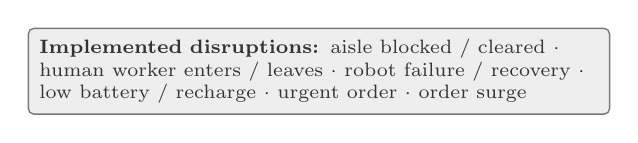
\begin{tikzpicture}
  \node[fboxgray,text width=7.1cm,font=\scriptsize,align=left,inner sep=4pt]
  {\textbf{Implemented disruptions:} aisle blocked / cleared $\cdot$ human worker enters / leaves
   $\cdot$ robot failure / recovery $\cdot$ low battery / recharge $\cdot$ urgent order $\cdot$ order surge};
\end{tikzpicture}
\end{column}

\begin{column}{0.43\textwidth}
\centering
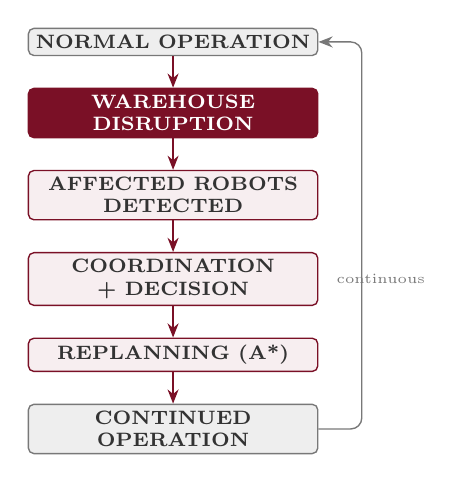
\begin{tikzpicture}[node distance=4.0mm]
  \node[fboxgray,text width=3.5cm] (n1) {NORMAL OPERATION};
  \node[fboxdark,text width=3.5cm,below=of n1] (n2) {WAREHOUSE DISRUPTION};
  \node[fbox,text width=3.5cm,below=of n2]     (n3) {AFFECTED ROBOTS DETECTED};
  \node[fbox,text width=3.5cm,below=of n3]     (n4) {COORDINATION + DECISION};
  \node[fbox,text width=3.5cm,below=of n4]     (n5) {REPLANNING (A*)};
  \node[fboxgray,text width=3.5cm,below=of n5] (n6) {CONTINUED OPERATION};

  \foreach \a/\b in {n1/n2,n2/n3,n3/n4,n4/n5,n5/n6}{\draw[arr] (\a) -- (\b);}

  \draw[arrgray,rounded corners] (n6.east) -- ++(0.55,0) |- (n1.east);
  \node[font=\tiny,text=MidGray,anchor=west] at ([xshift=3pt]n4.east) {continuous};
\end{tikzpicture}
\end{column}

\end{columns}
\end{frame}

%==============================================================
%  SLIDE 3 -- PEAS
%==============================================================
\begin{frame}{PEAS Specification}
\centering
\setlength{\tabcolsep}{4pt}
\renewcommand{\arraystretch}{1.25}
\scriptsize
\begin{tabular}{@{}L{1.85cm} L{11.6cm}@{}}
\toprule
\rowcolor{AmritaMaroon}
\hcell{Element} & \hcell{Instantiation in this project}\\
\midrule
\rowcolor{MaroonTint}
\peasrow{Performance} &
Orders completed (pending / active tracked separately) $\cdot$ \textbf{collisions (target 0)} $\cdot$
conflicts prevented $\cdot$ replans and reroutes per disruption $\cdot$ total travel distance $\cdot$
idle and waiting ticks $\cdot$ robot utilisation $=(\text{ticks}-\text{idle}-\text{wait})/\text{ticks}$\\

\peasrow{Environment} &
$22\times18$ discrete grid $\cdot$ 5 vertical aisles A1--A5 flanked by shelves $\cdot$ 3 horizontal
corridors $\cdot$ one pickup point per aisle $\cdot$ charging, packing, receiving and shipping stations
$\cdot$ 5 robots $\cdot$ human workers (safety radius 2) $\cdot$ blockable aisles $\cdot$ order stream
(auto every 80 ticks, plus urgent / surge)\newline
\textit{Properties:} discrete, dynamic, sequential, multi-agent, fully observable, deterministic (seed 42)\\

\rowcolor{MaroonTint}
\peasrow{Actuators} &
\textit{Robot:} move one cell (4-connected) $\cdot$ wait $\cdot$ stop $\cdot$ reroute $\cdot$ pick (5 ticks)
$\cdot$ deliver (4 ticks) $\cdot$ charge ($+2\%$ per tick up to $95\%$)\newline
\textit{Coordinator:} assign / reassign an order $\cdot$ reserve and release path cells $\cdot$ broadcast
messages to the fleet\\

\peasrow{Sensors} &
Own position, battery, status and remaining-path validity $\cdot$ cell walkability, blocked aisles,
human positions and safety radius $\cdot$ other robots' positions (congestion) $\cdot$ reservation-table
conflicts (vertex / edge-swap) $\cdot$ order queue with priority and waiting time $\cdot$ tick counter
$\cdot$ user-triggered command events\\
\bottomrule
\end{tabular}

\vspace{5pt}
{\scriptsize\color{MidGray} Grid layout, fleet size, cost weights and battery thresholds are all read from
\texttt{config/*.yaml} -- nothing is hard-coded.}
\end{frame}

%==============================================================
%  SLIDE 4 -- AGENTS
%==============================================================
\begin{frame}{Agents in the System}
\begin{columns}[T,onlytextwidth]

\begin{column}{0.56\textwidth}
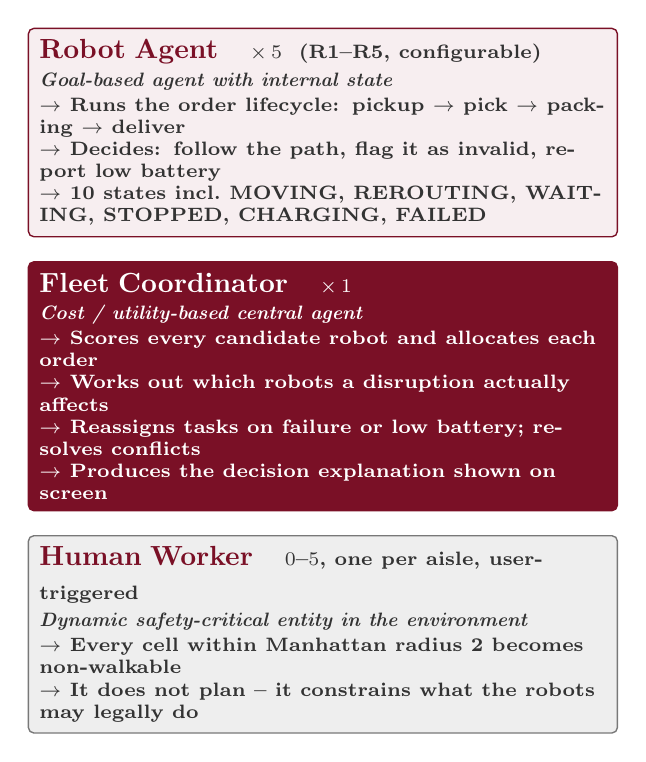
\begin{tikzpicture}
  \node[fbox,text width=7.2cm,align=left,inner sep=4pt] (a1)
  {\normalsize\lab{Robot Agent}\quad{\scriptsize $\times\,5$ \ (R1--R5, configurable)}\\[2pt]
   \scriptsize\textit{Goal-based agent with internal state}\\[1pt]
   \scriptsize $\to$ Runs the order lifecycle: pickup $\to$ pick $\to$ packing $\to$ deliver\\
   \scriptsize $\to$ Decides: follow the path, flag it as invalid, report low battery\\
   \scriptsize $\to$ 10 states incl.\ MOVING, REROUTING, WAITING, STOPPED, CHARGING, FAILED};

  \node[fboxdark,text width=7.2cm,align=left,inner sep=4pt,below=3mm of a1] (a2)
  {\normalsize\textbf{Fleet Coordinator}\quad{\scriptsize $\times\,1$}\\[2pt]
   \scriptsize\textit{Cost / utility-based central agent}\\[1pt]
   \scriptsize $\to$ Scores every candidate robot and allocates each order\\
   \scriptsize $\to$ Works out which robots a disruption actually affects\\
   \scriptsize $\to$ Reassigns tasks on failure or low battery; resolves conflicts\\
   \scriptsize $\to$ Produces the decision explanation shown on screen};

  \node[fboxgray,text width=7.2cm,align=left,inner sep=4pt,below=3mm of a2] (a3)
  {\normalsize\lab{Human Worker}\quad{\scriptsize $0$--$5$, one per aisle, user-triggered}\\[2pt]
   \scriptsize\textit{Dynamic safety-critical entity in the environment}\\[1pt]
   \scriptsize $\to$ Every cell within Manhattan radius 2 becomes non-walkable\\
   \scriptsize $\to$ It does not plan -- it constrains what the robots may legally do};
\end{tikzpicture}
\end{column}

\begin{column}{0.42\textwidth}
\centering
\vspace{1mm}
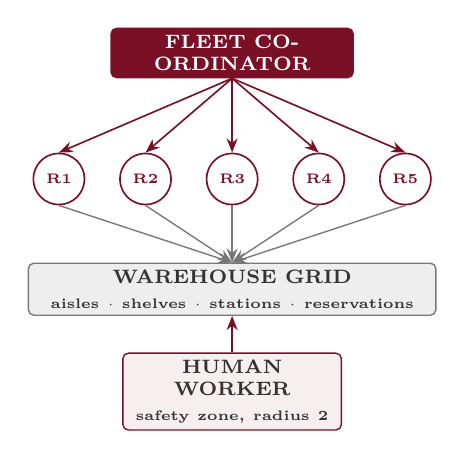
\begin{tikzpicture}
  \node[fboxdark,text width=2.9cm] at (0,0) (co) {FLEET COORDINATOR};

  \foreach \i/\x in {1/-2.2,2/-1.1,3/0,4/1.1,5/2.2}{
    \node[bot] (r\i) at (\x,-1.6) {R\i};
    \draw[arr] (co.south) -- (r\i.north);
  }

  \node[fboxgray,text width=5.0cm] at (0,-3.0) (wh)
    {WAREHOUSE GRID\\[1pt]{\tiny aisles $\cdot$ shelves $\cdot$ stations $\cdot$ reservations}};
  \foreach \i in {1,...,5}{\draw[arrgray] (r\i.south) -- (wh.north);}

  \node[fbox,text width=2.6cm] at (0,-4.3) (hu)
    {HUMAN WORKER\\[1pt]{\tiny safety zone, radius 2}};
  \draw[arr] (hu.north) -- (wh.south);
\end{tikzpicture}

\vspace{1mm}
{\scriptsize\color{MidGray} Coordinator \emph{assigns}; robots \emph{report}; the human
\emph{constrains}. The demo runs \textbf{1 coordinator}, \textbf{5 robots}, \textbf{5 aisles}.}
\end{column}

\end{columns}
\end{frame}

%==============================================================
%  SLIDE 5 -- SCENARIOS AND SOLUTIONS
%==============================================================
\begin{frame}{Scenarios and Corresponding Solutions}
\centering
\vspace{-1mm}

\begin{tikzpicture}
 \node[fboxgray,text width=12.6cm,font=\tiny,inner sep=2pt]
 {TRIGGER $\;\to\;$ EFFECT ON WAREHOUSE $\;\to\;$ SYSTEM RESPONSE $\;\to\;$ AI LOGIC USED};
\end{tikzpicture}

\vspace{1.5mm}
\setlength{\tabcolsep}{3pt}
\renewcommand{\arraystretch}{1.05}
\scriptsize
\begin{tabular}{@{}L{2.3cm} L{2.9cm} L{4.5cm} L{3.0cm}@{}}
\toprule
\rowcolor{AmritaMaroon}
\hcell{Trigger} & \hcell{Effect} & \hcell{System response} & \hcell{AI logic}\\
\midrule
\rowcolor{MaroonTint}
\cmd{BLOCK A3} & Aisle cells non-walkable &
Robots whose path crosses it are detected; reservations cleared; REROUTING, or WAITING if no route exists &
A* replanning + reservation update\\

\cmd{UNBLOCK A3} & Aisle walkable again &
Only \emph{waiting} robots re-evaluate; others continue &
Selective replanning\\

\rowcolor{MaroonTint}
\cmd{HUMAN ENTER A2} & Safety zone, radius 2 &
Robot inside the zone STOPS; a robot whose path crosses it REROUTES &
Safety as a hard constraint\\

\cmd{HUMAN REMOVE A2} & Safety zone cleared &
Stopped and waiting robots replan and resume &
Constraint relaxation\\

\rowcolor{MaroonTint}
\cmd{FAIL R3} & Robot frozen; reservations released &
Order recovered; candidates scored on distance, battery and workload; best robot takes it &
Cost-based reassignment + A*\\

\cmd{RECOVER R3} & Robot returns to IDLE &
Rejected unless truly FAILED; then rejoins the allocation pool &
Guarded state transition\\

\rowcolor{MaroonTint}
\cmd{LOW BATTERY R3} & Battery forced to $8\%$ &
Battery weighed against the energy the task needs; routed to the charger; order reassigned &
Utility comparison + A*\\

\cmd{URGENT ORDER}\newline\cmd{ORDER SURGE} & Priority-10 order / 5 new orders &
Queue re-sorted by effective priority; allocation runs at once &
Priority scheduling with aging\\
\bottomrule
\end{tabular}

\vspace{2pt}
{\scriptsize\color{MidGray} Every trigger works for \emph{any} configured aisle (A1--A5) or robot (R1--R5).}
\end{frame}

%==============================================================
%  SLIDE 6 -- AI DECISION-MAKING ARCHITECTURE
%==============================================================
\begin{frame}{AI Decision-Making Architecture}
\begin{columns}[T,onlytextwidth]

\begin{column}{0.34\textwidth}
\centering
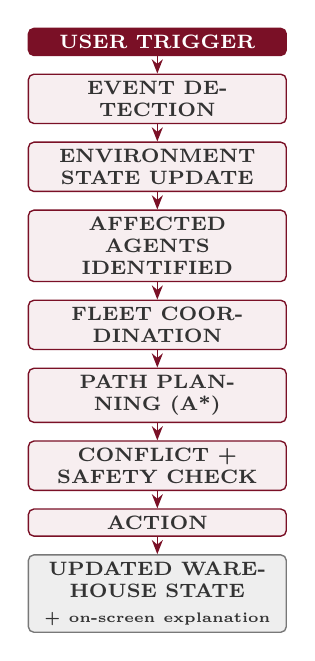
\begin{tikzpicture}[node distance=2.2mm]
  \node[fboxdark,text width=3.1cm] (p1) {USER TRIGGER};
  \node[fbox,text width=3.1cm,below=of p1] (p2) {EVENT DETECTION};
  \node[fbox,text width=3.1cm,below=of p2] (p3) {ENVIRONMENT STATE UPDATE};
  \node[fbox,text width=3.1cm,below=of p3] (p4) {AFFECTED AGENTS IDENTIFIED};
  \node[fbox,text width=3.1cm,below=of p4] (p5) {FLEET COORDINATION};
  \node[fbox,text width=3.1cm,below=of p5] (p6) {PATH PLANNING (A*)};
  \node[fbox,text width=3.1cm,below=of p6] (p7) {CONFLICT + SAFETY CHECK};
  \node[fbox,text width=3.1cm,below=of p7] (p8) {ACTION};
  \node[fboxgray,text width=3.1cm,below=of p8] (p9)
       {UPDATED WAREHOUSE STATE\\[1pt]{\tiny + on-screen explanation}};
  \foreach \a/\b in {p1/p2,p2/p3,p3/p4,p4/p5,p5/p6,p6/p7,p7/p8,p8/p9}{\draw[arr] (\a) -- (\b);}
\end{tikzpicture}
\end{column}

\begin{column}{0.64\textwidth}
\scriptsize

\begin{block}{\small 1.\ Path planning -- A* search}
\vspace{-5pt}
\[ f(n)=g(n)+h(n) \]
\vspace{-15pt}
\begin{itemize}
  \item $g(n)=\sum\big(1+3.0\cdot\mathrm{congestion}(n)\big)$ -- steps, penalised near other robots
  \item $h(n)=$ Manhattan distance (admissible on a 4-connected grid)
  \item Blocked aisles and human safety zones are removed from the walkable set, so A* can never
        return an unsafe path
\end{itemize}
\end{block}

\vspace{-3pt}
\begin{block}{\small 2.\ Task allocation -- cost minimisation}
\vspace{-8pt}
\[ \mathrm{cost}=d+2.0\,w+3.0\,c+0.5\max(0,30-b)+1.5\,t-3.0\,p_{\mathrm{eff}} \]
\vspace{-15pt}
\[ p_{\mathrm{eff}}=\mathrm{priority}+0.1\,t \qquad \textit{(priority aging)} \]
\vspace{-7pt}
\begin{itemize}
  \item $d$ distance, $w$ workload, $c$ congestion, $b$ battery, $t$ waiting time -- lowest cost wins
\end{itemize}
\end{block}

\vspace{-3pt}
\begin{block}{\small 3.\ Collision avoidance and dynamic replanning}
\vspace{-4pt}
\begin{itemize}
  \item Space--time \textbf{reservation table}: $(\mathrm{cell},t)\to\mathrm{robot}$, detecting
        \textsc{vertex} and \textsc{edge-swap} conflicts
  \item Conflicting cells are fed back into A* as a forbidden set; a per-tick check makes one robot \textsc{wait}
  \item Replanning is \textbf{localised} -- only robots whose remaining path became invalid are replanned
\end{itemize}
\end{block}

\end{column}
\end{columns}
\end{frame}

%==============================================================
%  SLIDE 7 -- DEMONSTRATION / RESULTS / KEY TAKEAWAYS
%==============================================================
\begin{frame}{Demonstration and Key Takeaways}

\centering
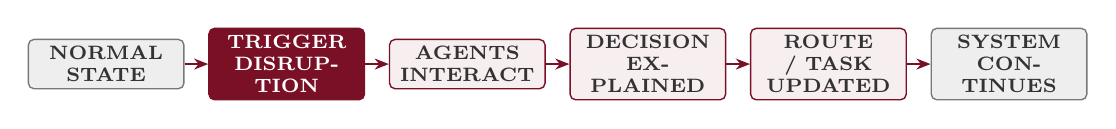
\begin{tikzpicture}[node distance=3.0mm]
  \node[fboxgray,text width=1.8cm] (d1) {NORMAL STATE};
  \node[fboxdark,text width=1.8cm,right=of d1] (d2) {TRIGGER DISRUPTION};
  \node[fbox,text width=1.8cm,right=of d2] (d3) {AGENTS INTERACT};
  \node[fbox,text width=1.8cm,right=of d3] (d4) {DECISION EXPLAINED};
  \node[fbox,text width=1.8cm,right=of d4] (d5) {ROUTE / TASK UPDATED};
  \node[fboxgray,text width=1.8cm,right=of d5] (d6) {SYSTEM CONTINUES};
  \foreach \a/\b in {d1/d2,d2/d3,d3/d4,d4/d5,d5/d6}{\draw[arr] (\a) -- (\b);}
\end{tikzpicture}

\vspace{3mm}
\begin{columns}[T,onlytextwidth]

\begin{column}{0.55\textwidth}
{\footnotesize\lab{Demonstrated capabilities}}
\vspace{1mm}
\begin{itemize}\scriptsize\setlength{\itemsep}{2pt}
  \item \tick\ Every aisle and robot triggerable live -- typed commands \emph{and} context-sensitive
        buttons generated from the configuration
  \item \tick\ Localised disruption: unaffected robots keep working
  \item \tick\ Robot failure $\to$ order recovered and reassigned, never lost
  \item \tick\ Human-aware navigation: safety enforced as a hard constraint
  \item \tick\ Battery-aware behaviour: charge-versus-continue decision
  \item \tick\ Explainable output: agent dialogue, cost breakdown and the algorithm named for every event
  \item \tick\ Invalid commands rejected safely -- unknown IDs list the valid ones, \cmd{RECOVER}
        requires a FAILED robot; the simulation never crashes
  \item \tick\ Deterministic replay (seed 42) -- the same demonstration every time
\end{itemize}
\end{column}

\begin{column}{0.43\textwidth}
{\footnotesize\lab{Instrumented metrics}} {\scriptsize(live dashboard and \cmd{TERMINATE} summary)}
\vspace{2mm}

\setlength{\tabcolsep}{3pt}
\renewcommand{\arraystretch}{1.12}
\scriptsize
\begin{tabular}{@{}L{2.9cm} L{2.4cm}@{}}
\toprule
\rowcolor{AmritaMaroon}
\hcell{Metric} & \hcell{What it shows}\\
\midrule
\rowcolor{MaroonTint}
Orders completed / pending & Throughput\\
Replans, reroutes & Adaptation effort\\
\rowcolor{MaroonTint}
Conflicts prevented & Coordination quality\\
Collisions & Safety (target 0)\\
\rowcolor{MaroonTint}
Total distance & Travel efficiency\\
Idle / waiting ticks & Robot utilisation\\
\bottomrule
\end{tabular}

\vspace{2mm}
{\scriptsize\color{MidGray} These counters are produced at run time by the live simulation and read
off the screen during the demonstration.}
\end{column}
\end{columns}

\vspace{3mm}
\centering

\begin{tikzpicture}
 \node[fboxdark,text width=12.8cm,font=\scriptsize,inner sep=3.5pt]
 {Takeaway: safety outranks throughput $\;\cdot\;$ a local disruption must not trigger a global replan
  $\;\cdot\;$ every decision is explained, not merely executed};
\end{tikzpicture}
\end{frame}

%==============================================================
%  SLIDE 8 -- THANK YOU
%==============================================================
\begin{frame}[plain]
\begin{tikzpicture}[remember picture,overlay]
  \fill[AmritaMaroon] (current page.north west) rectangle (current page.south east);
  \fill[MaroonLight]  ([yshift=-4.42cm]current page.north west) rectangle
                      ([yshift=-4.55cm]current page.north east);

  \node[text=white,font=\fontsize{46}{50}\selectfont\bfseries]
    at ([yshift=1.25cm]current page.center) {THANK YOU};
  \node[text=MaroonTint,font=\Large]
    at ([yshift=-0.35cm]current page.center) {Questions?};
  \node[text=white,font=\small\bfseries]
    at ([yshift=-1.85cm]current page.center) {Warehouse That Reroutes Itself};
  \node[text=MaroonTint,font=\footnotesize]
    at ([yshift=-2.35cm]current page.center) {Group 10};
\end{tikzpicture}
\end{frame}

\end{document}
